\documentclass[a4paper]{article}

%% Language and font encodings
\usepackage[english]{babel}
\usepackage[utf8x]{inputenc}
\usepackage[T1]{fontenc}

%% Sets page size and margins
\usepackage[a4paper,top=3cm,bottom=2cm,left=3cm,right=3cm,marginparwidth=1.75cm]{geometry}

%% Useful packages
\usepackage{graphicx}
\usepackage{float}
\usepackage[colorlinks=true, allcolors=blue]{hyperref}

\title{%
  Advanced Topics in Computer Science \\
  \large Celestial Similarity Index \\ }
 
\title{%
  Advanced Topics in Computer Science - University of Padova \\
  \large Secure Computation Report: Celestial Similarity Index}

\author{Marco Casagrande}

\begin{document}
\maketitle

\section{Overview}

\subsection{Assignment}

The assignment:

\begin{itemize}
    \item Install the Obliv-C library;
    \item Think of a two-party application that requires data privacy;
    \item Implement the algorithm with Obliv-C;
    \item Run it and collect some results (running time);
    \item Put everything in a report.
\end{itemize}

\subsection{Installing Obliv-C}

I downloaded the Ubuntu 18.04.1 LTS 64bit ISO and installed it in Oracle VirtualBox. Following Obliv-C \href{https://oblivc.org/tutorial/}{guide}, while installing a few more dependencies, I was able run the test applications smoothly.

\subsection{Learning Obliv-C}

Following along the tutorial on \href{https://oblivc.org/tutorial/}{guide} was useful but I found it not in depth enough. I then started looking at the code of the various test applications to understand the logic behind Obliv-C features usage. The \href{https://oblivc.org/tutorial/}{documentation} was really helpful but still I'd have preferred more detail.

\subsection{Generating the idea}

Year 2XXX. Advanced technology made possible to create efficient starships and explore the universe. Companies are sending probes to scan celestial bodies, hoping for valuable discoveries. No company wants to share precise information, but is willing to disclose a little if it can confirm the rightfulness of its data. \\ \href{http://phl.upr.edu/projects/earth-similarity-index-esi}{Earth Similarity Index (ESI)} corresponds to how a celestial body is similar to the Earth. Using the same principle, it is possible to compare any celestial body, in fact providing the Celestial Similarity Index (fantasy name). \\
Many scenarios could be invented, for example:

\begin{itemize}
    \item Comparing two different samples, from different companies, from the same celestial body and verifying if the Similarity Index is close, thus analyzing the data rightfulness.
    \item Analyzing the data rightfulness of an entire sector of celestial bodies. If a sector of celestial bodies presents 80\% of similar features, then comparing the Similarity Index of a random celestial body from Company 1 to the SI of a random celestial body from Company 2 will most likely provide an 80\% match on SI from randomly paired celestial bodies.
\end{itemize}

My purpose was implementing a simple application that could resolve those scenarios.

\subsection{The idea}

My application involves two parties. Both of them have to input a celestial body name (aesthetics only), a stellar flux value and a radius value. The application then will output the Similarity Index between the two celestial bodies.

\section{Implementation}

\subsection{Setup}

I started creating test/oblivc/csi copying the entirety of test/oblivc/editdist (Levenshtein distance) application folder, because of its code readability and compatibility with my idea. Many steps of a new implementation (input formatting, TCP connection, Yao's protocol invocation...) are almost standardized in those test examples so why reinventing them? 

\subsection{File explanation}

\subsubsection{si.h}

Header file. Declares the struct protocolIO, the main function compareIO and other more generic functions (implemented in test/oblivc/common or test/oblivc/si/si.c).

\subsubsection{si.c}

C language file. Implements some generic functions, gathers inputs, prepares data structures, creates a TCP connection between parties, tracks time, calls execYaoProtocol(\&pd,compareSI,\&io), cleans up and prints the revealed output.

\subsubsection{si.oc}

C language file using Obliv-C library. Implements computeSI() and the various oblivious functions it requires to operate. Shares the oblivious parameters about Stellar Flux and Radius, uses them to compute the Similarity Index between the celestial bodies chosen by the two parties. Finally, reveals the output and prints the number of gates needed for the Yao's garbled circuit instantiation.

\subsection{Code overview}

The code is really simple. The execution is started in si.c, gathering inputs, preparing data structures, tracking time and creating a TCP connection between parties. It continues in si.oc after calling execYaoProtocol(\&pd,compareSI,\&io), where the Obliv-C library operates. The call revealOblivFloat(\&io->si,osi,0); reveals the output to both parties so the execution ends in si.c, after some cleanup and the output print. \\
For more in depth explanation, comments can be found throughout all the code.

\section{Running the code}

The code is run almost like any other test application.

\begin{figure}[H]
  \centering
  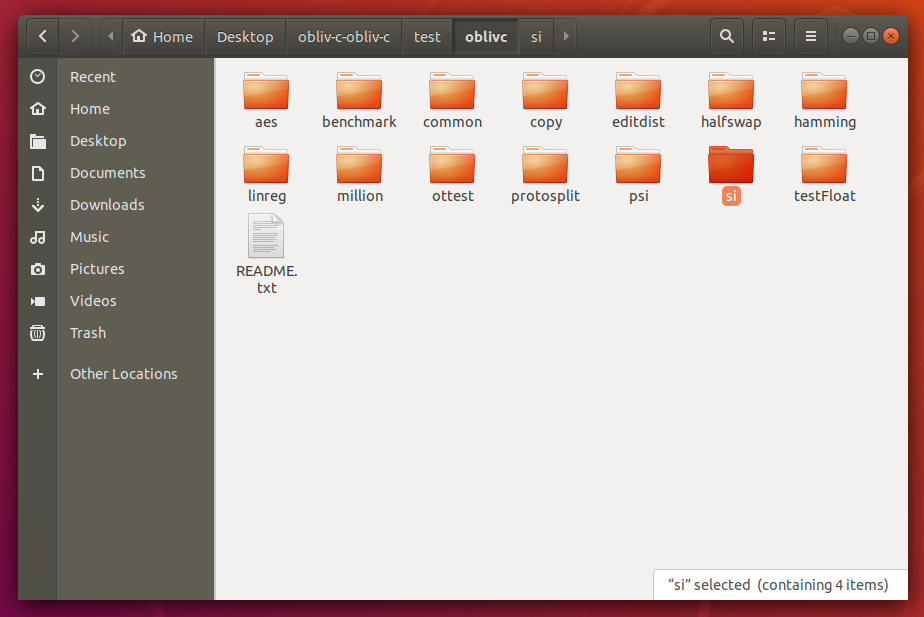
\includegraphics[width=0.8\textwidth]{testfolder.png}
  \caption{Download and extract the folder into: [Obliv-C folder]/test/oblivc}
\end{figure}

\begin{figure}[H]
  \centering
  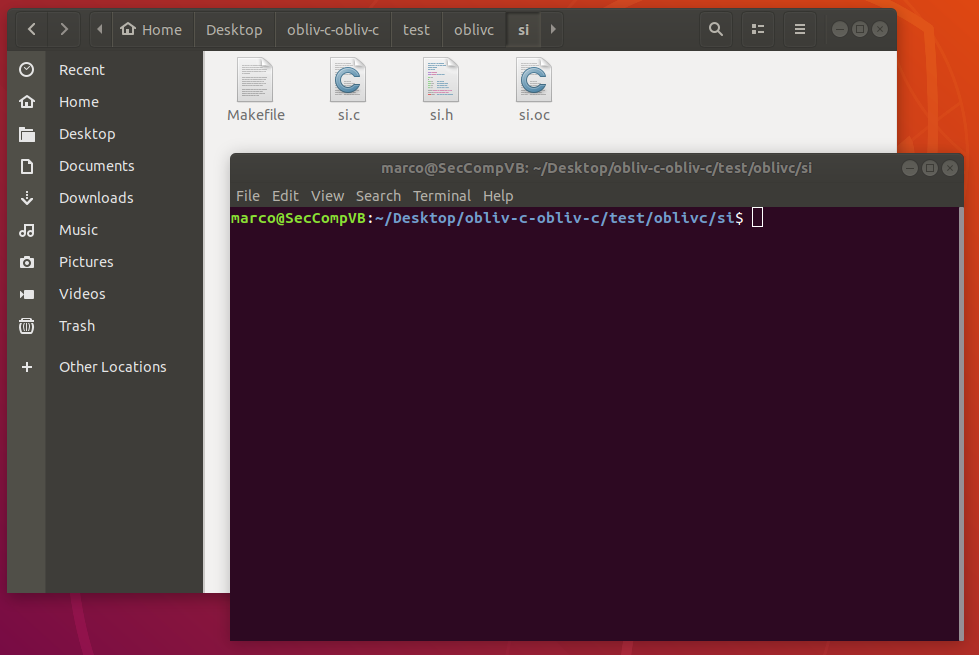
\includegraphics[width=0.8\textwidth]{terminal.png}
  \caption{Reach inside the si folder and open the terminal from there, or just open a normal terminal and navigate to the aforementioned place}
\end{figure}

\begin{figure}[H]
  \centering
  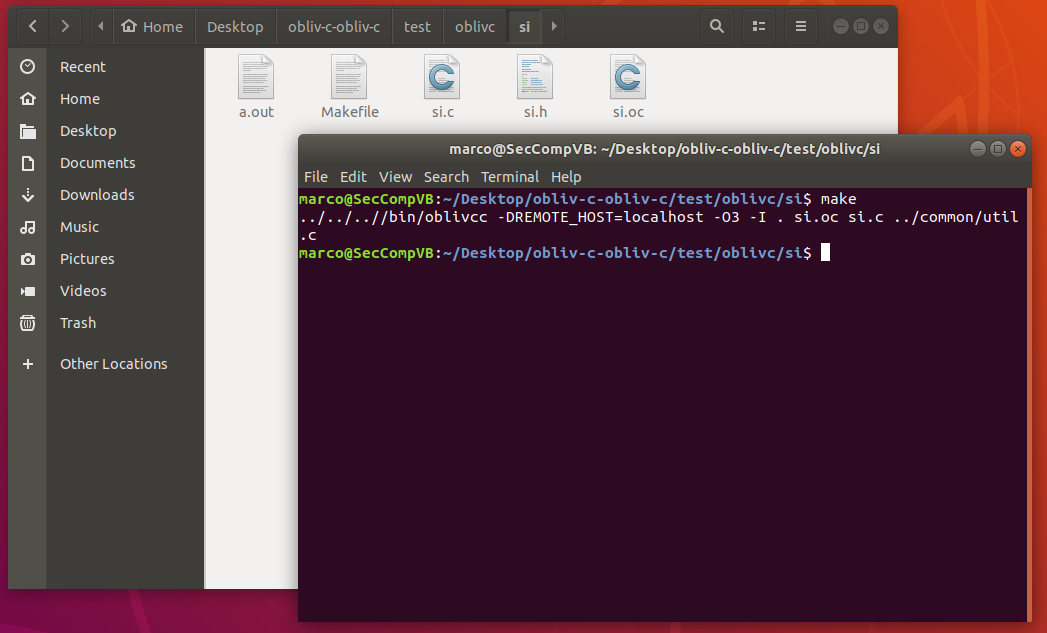
\includegraphics[width=0.8\textwidth]{make.png}
  \caption{Run the make command}
\end{figure}

\begin{figure}[H]
  \centering
  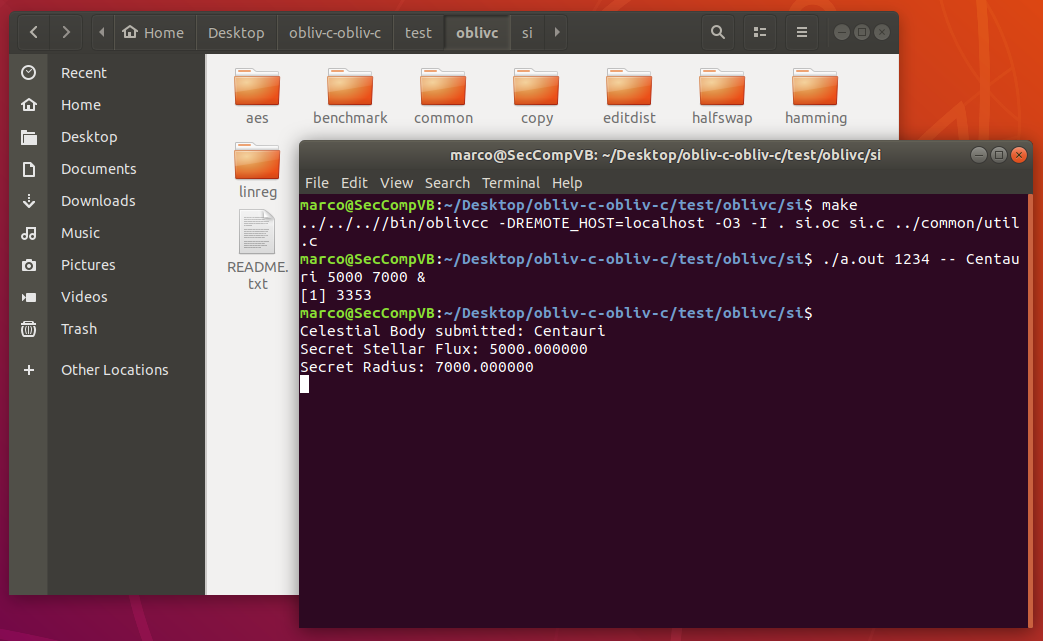
\includegraphics[width=0.8\textwidth]{generator.png}
  \caption{Run a command with the format "<a.out location> <port> <--> <celestial body> <stellar flux> <radius> \&"}
\end{figure}

\begin{figure}[H]
  \centering
  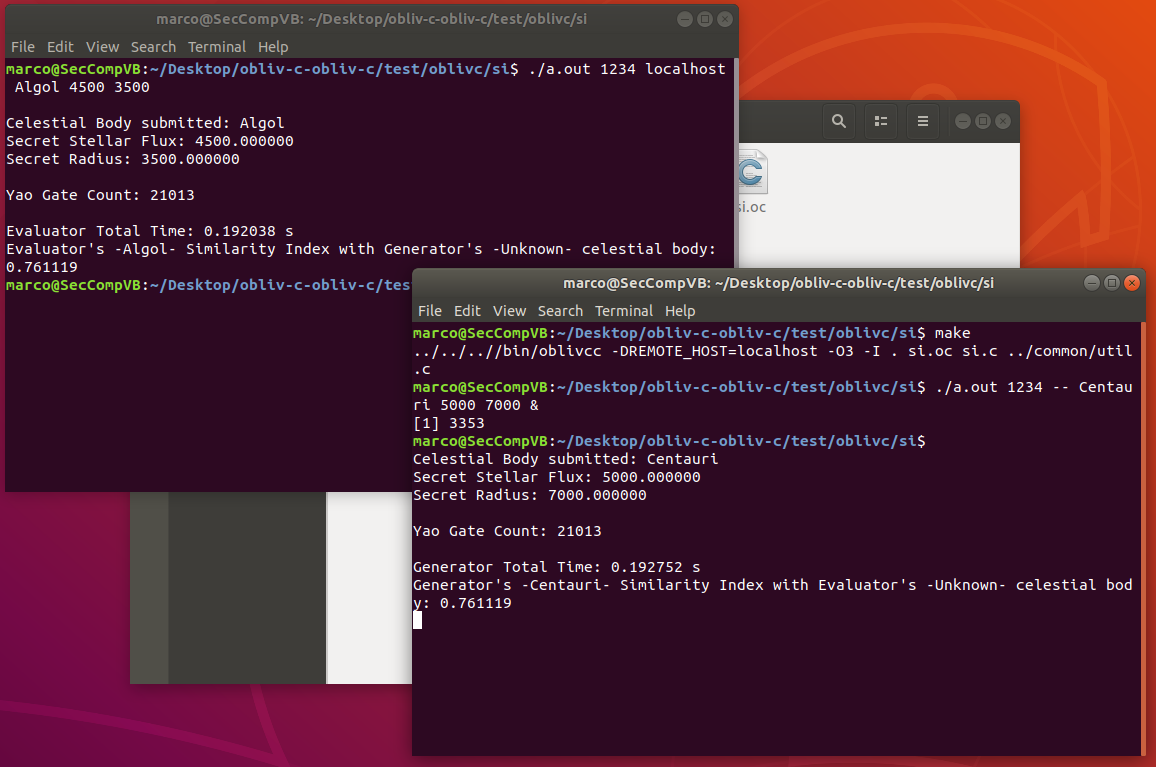
\includegraphics[width=0.8\textwidth]{evaluator.png}
  \caption{Run a command with the format "<a.out location> <port> <remote\_host> <celestial body> <stellar flux> <radius>". At this point, both parties will have submitted their data and the output will be computed and revealed to both of them}
\end{figure}

Of course the code can be run with any parameter that follows the input format (and protocolIO correct typing).

\section{Challenges}

\subsection{Oblivious math.h}

Originally I wanted to used the \href{http://phl.upr.edu/projects/earth-similarity-index-esi}{ESI from Radius, Density, Escape Velocity, and Surface Temperature} formula. At first, I thought using math.h (specifically for abs(float) and pow(float,float) operations) but I couldn't even compile the code. An \href{https://github.com/samee/obliv-c/issues/48}{issue} on github granted me a workaround: adding \#undef \_\_HAVE\_DISTINCT\_FLOAT128 before including math.h. Unfortunately, after working on abs(float) I acknowledged the need of using an oblivious abs(float), because the parameter was oblivious. Still, that implementation was trivial. But for the pow(float,float) it looked too daunting to elaborate an oblivious implementation. So I fell back to the \href{http://phl.upr.edu/projects/earth-similarity-index-esi}{ESI from Stellar Flux and Radius} formula.

\subsection{Oblivious square root algorithm}

The \href{http://phl.upr.edu/projects/earth-similarity-index-esi}{ESI from Stellar Flux and Radius} formula was much easier to implement. Most oblivious operations were trivial (summation, subtraction, division, square...). The difficult one was the oblivious sqrt(float). As I already stated, I couldn't use math.h operations because they are not oblivious. I could take two approaches from there:

\begin{itemize}
    \item Revealing the intermediate result to both parties;
    \item Implementing an oblivious sqrt(float) function.
\end{itemize}

The first approach of revealing the intermediate result to both parties would transform the oblivious parameter into a non oblivious parameter, allowing the usage of math.h sqrt(float). It would be easy to implement but would almost instantly breach privacy. When the final output is a comparative value (the Similarity Index), backtracking the Stellar Flux and Radius of the other party is difficult (apart from SI ~= 1.0). Disclosing an intermediate, non-comparative, value would lead to easily reverse engineering the Stellar Flux and Radius of the other party.
\\
\\
The second approach of implementing an oblivious sqrt(float) function would be ideal but requires to find an adequate algorithm. After some search and failed implementations, I found my answer (of course) on a Stackoverflow discussion about \href{https://stackoverflow.com/questions/28264277/square-root-union-and-bit-shift}{Square root union and Bit Shift}. After some trials, it looks like it's working correctly, even sporting an high precision. 

\section{Conclusion}

SI is a simple example about secure computing. In this scenario, two parties are gathering information (Stellar Flux and Radius) about celestial bodies, sharing them among themselves but without any disclosure and both collecting the Similarity Index as the only output. \\
The final result was good: the code is working and returning the right outputs, the code is simple and readable, the execution time isn't massively slowed down by the usage of Yao's garbled circuits. \\
I gained knowledge about the Obliv-C library, and even more:

\begin{itemize}
    \item how to arrange, configure, write, compile and run Obliv-C code;
    \item how to use the obliv keyword (variables, if, for);
    \item how to use Obliv-C API documentation (both C functions and Obliv-C functions);
    \item how to implement oblivious algorithms starting from their non-oblivious counterpart;
    \item and lots of information about algorithms, programming, logic and astronomy!
\end{itemize}

\end{document}